\documentclass{article}
\RequirePackage[a4paper, total={6in, 8in}]{geometry}
\RequirePackage{setspace}
\RequirePackage{floatrow}
\RequirePackage[hidelinks]{hyperref}
\RequirePackage{enumitem}
\RequirePackage{calc}
\RequirePackage{amsmath}
\RequirePackage{textcomp, gensymb}
% figures
\RequirePackage{graphicx}
\graphicspath{ {images/} }
\RequirePackage{subcaption}
% biblio
\RequirePackage[nottoc,notlot,notlof,numbib]{tocbibind}
\RequirePackage{natbib}
\onehalfspacing
% code
\RequirePackage{color}
\bibliographystyle{agsm}

\newcounter{qn_no}
\newenvironment*{qn}[1]{
    \stepcounter{qn_no}
    \noindent{\color{red}\Alph{qn_no}) #1}
    \par
}{\vspace{1em}\hrule\vspace{1em}}

\begin{document}

\begin{center}
    {\Huge \bfseries Computing CW -- Summary}
\end{center}

\hspace{-1cm}
Students: Dylan CHUA -- 02131550, Chong Hui FENG -- 02015459 \hfill Path: B, Words: 999/1000
\hspace{-1cm}
\vspace{1em}
\hrule

\vspace{1em}

\begin{qn}{What physics are you trying to model and analyse? (Describe clearly, in words, what physical phenomenon you wish to analyse)}
    The Black-Scholes model has been chosen to predict the dynamics of a financial market. As the stock price is random and follows a Brownian motion with drift, there is a range of possibilities of the stock price at a specified date in the future. In the market there is an option on the stock, which gives the buyer of the option the possibility to buy the stock at the strike price in the future. There exists a fair value of the option which eliminates risk. The value is dependent on the time to expiry t and stock price S, which can be described using a PDE.
\end{qn}

\begin{qn}{What PDE are you trying to solve, associated with the Physics described in A? (write the PDE)}
    The PDE associated with the Black-Scholes model is the Black-Scholes equation, which is a convection-diffusion parabolic type PDE – first-order in time, second-order in stock price (with non-zero first and second derivatives).

    \begin{equation}
        \frac{\partial V}{\partial t} + \frac{1}{2}\sigma^2S^2\frac{\partial^2 V}{\partial S^2} + rS\frac{\partial V}{\partial S} - rV = 0
    \end{equation}
    
    Based on market conditions (risk-free interest rate $r$, volatility $\sigma$ and strike price $K$), theoretical estimates for European-style options ($V$) can be obtained for different values of stock price $S$ and time to expiry $t$.
\end{qn}

\begin{qn}{Boundary value and/or initial values for my specific problem: (be CONSISTENT with what you wrote in A)}
Since the PDE is first-order in time and second-order in stock price, one condition in time and two boundary conditions in price are needed. The Black-Scholes equation is a backwards parabolic equation, meaning the final condition is known and the equation is solved for $t < T$.

\underline{Final Condition}
\begin{equation}
    V\left(S,T\right)=\max\{S-K,0\}
    \label{eqn:finalcond}
\end{equation}

The final value of the call option at time $T$ is simply the profit earned upon maturity of the option. However, the profit cannot be negative hence $\max\{S-K,0\}$ is needed to ensure $V\left(S,T\right)>0$ for all $S$.

\underline{Boundary Condition 1}
\begin{equation}
    V\left(0,t\right)=0\ for\ all\ t
\end{equation}

The call option value $V$ when stock price $S$ is zero (worthless) will also be zero.

\underline{Boundary Condition 2}
\begin{equation}
    V\left(S,t\right)\rightarrow S-Ke^{-r(T-t)}\ as\ S\ \rightarrow \infty 
\end{equation}
As $S\ \rightarrow \infty$, it becomes ever more likely that the option will be exercised hence the magnitude of the strike price becomes less important (discounted). The option price thus becomes the stock price $S$ minus the discounted strike price $K$; the “discount” is applied by the $e^{-r(T-t)}$\ term which leads to a temporal decay of $K$.

\end{qn}

\begin{qn}{What numerical method are you going to deploy and why? (Describe, in words, which method you intend to apply and why you have chosen it as opposed to other alternatives)}
An explicit finite difference method and an implicit method (Crank-Nicolson) were used. Out of all the implicit methods, Crank-Nicolson was chosen as it is one of the most popular finite difference schemes used to approximate the Black-Scholes PDE \citep{duffy}.
\end{qn}

\begin{qn}{I am going to discretise my PDE as the following (show the steps from continuous to discrete equation and boundary/initial conditions:}
Both methods employ a forward difference in time, and a central difference in stock price. To convert the PDE from a backwards to a forwards equation, a time substitution can be made by:

\begin{equation}
    \begin{aligned}
    \tau & = T - t \\
    \frac{\partial V}{\partial t} & = \frac{\partial V}{\partial \tau}\frac{\partial \tau}{\partial t} \\
    & = -\frac{\partial V}{\partial \tau}
    \end{aligned}
\end{equation}

and hence,

\begin{equation}
    -V_\tau + \frac{1}{2}\sigma^2S^2V_{SS} + rSV_S - rV = 0
\end{equation}

The condition in Eqn. \ref{eqn:finalcond} therefore turns into an initial condition:

\begin{equation}
    V\left(S,0\right)=\max\{S-K,0\}
\end{equation}

The other boundary conditions become:

\begin{equation}
    V\left(0,\tau\right)=0\ for\ all\ \tau
\end{equation}

\begin{equation}
    V\left(S,\tau\right)\rightarrow S-Ke^{-r\tau}\ as\ S\ \rightarrow \infty 
\end{equation}

With a mesh size in $S$ of $h$ and time step of $k$, $V_\tau$ is defined by the forward difference method:

\begin{equation}
    V_\tau = \frac{1}{k} \left(V_{S,\tau+k} - V_{S,\tau}\right)
\end{equation}

In the explicit method, $V_{SS}$ and $V_S$ are transformed using the central difference method:

\begin{equation}
    V_S = \frac{1}{2h} \left(V_{S+h,\tau} - V_{S-h,\tau}\right)
\end{equation}

\begin{equation}
    V_{SS} = \frac{1}{h^2} \left(V_{S+h,\tau} - 2V_{S,\tau} + V_{S-h,\tau}\right)
\end{equation}

Substituting back into the PDE,

\begin{equation}
    -\frac{V_{S,\tau+k} - V_{S,\tau}}{k} + \frac{\sigma^2S^2}{2h^2} \left(V_{S+h,\tau} - 2V_{S,\tau} + V_{S-h,\tau}\right) + \frac{rS}{h} \frac{V_{S+h,\tau} - V_{S-h,\tau}}{2} - rV_{S,\tau} = 0
\end{equation}

$V_{S,\tau+k}$ can thus be expressed explicitly in terms of $V_{S-h,\tau}$, $V_{S,\tau}$ and $V_{S+h,\tau}$. An iterative approach can be taken to iterate through the time steps and evaluating $V_{S,\tau+k}$ based on the previous time step.

In the implicit Crank-Nicolson method, $V_{SS}$, $V_S$ and $V$ are averaged by:

\begin{equation}
    V_S = \frac{1}{4h} \left(V_{S+h,\tau+k} - V_{S-h,\tau+k} + V_{S+h,\tau} - V_{S-h,\tau}\right)
\end{equation}

\begin{equation}
    V_{SS} = \frac{1}{2h^2} \left(V_{S+h,\tau+k} - 2V_{S,\tau+k} + V_{S-h,\tau+k} + V_{S+h,\tau} - 2V_{S,\tau} + V_{S-h,\tau}\right)
\end{equation}

\begin{equation}
    V = \frac{1}{2} \left(V_{S,\tau+k} + V_{S,\tau}\right)
\end{equation}

Substituting back into the PDE,

\begin{equation}
    \begin{aligned}
    &-\frac{V_{S,\tau+k} - V_{S,\tau}}{k}  \\& + \frac{\sigma^2S^2}{2h^2}\frac{V_{S+h,\tau+k} - 2V_{S,\tau+k} + V_{S-h,\tau+k} + V_{S+h,\tau} - 2V_{S,\tau} + V_{S-h,\tau}}{2} \\& + \frac{rS}{h}\frac{V_{S+h,\tau+k} - V_{S-h,\tau+k} + V_{S+h,\tau} - V_{S-h,\tau}}{4} \\& - r\frac{V_{S,\tau+k} + V_{S,\tau}}{2} \\& = 0
    \end{aligned}
\end{equation}

This is implicit as $V_{S,\tau+k}$ is dependent on $V_{S-h,\tau+k}$ and $V_{S+h,\tau+k}$. An iterative approach can be taken to iterate through the time steps, and at each time step, a system of equations can be initiated and solved by linear algebra.

\end{qn}

\begin{qn}{Plot the numerical results comprehensively and discuss them (discuss how the results describe the physics and comment on any discrepancies or unexpected behaviours). Use multiple types of visual graphs. Present and discuss any outcomes of the grid analysis, as requested in Task 9, too.}

\begin{figure}[h]
    \centering
    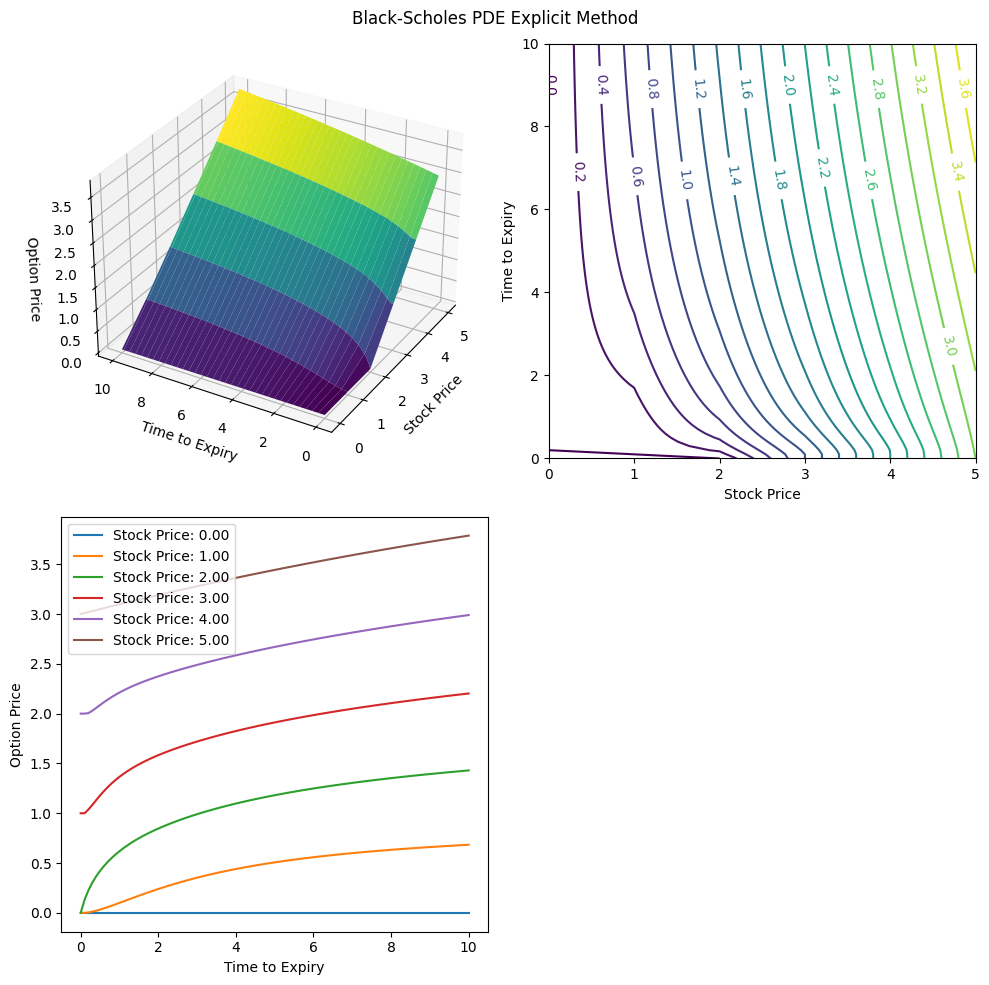
\includegraphics[width=0.8\textwidth]{explicit}
    \caption{Call option values using explicit method}
    \label{fig:explicit}
\end{figure}

\begin{figure}[h]
    \centering
    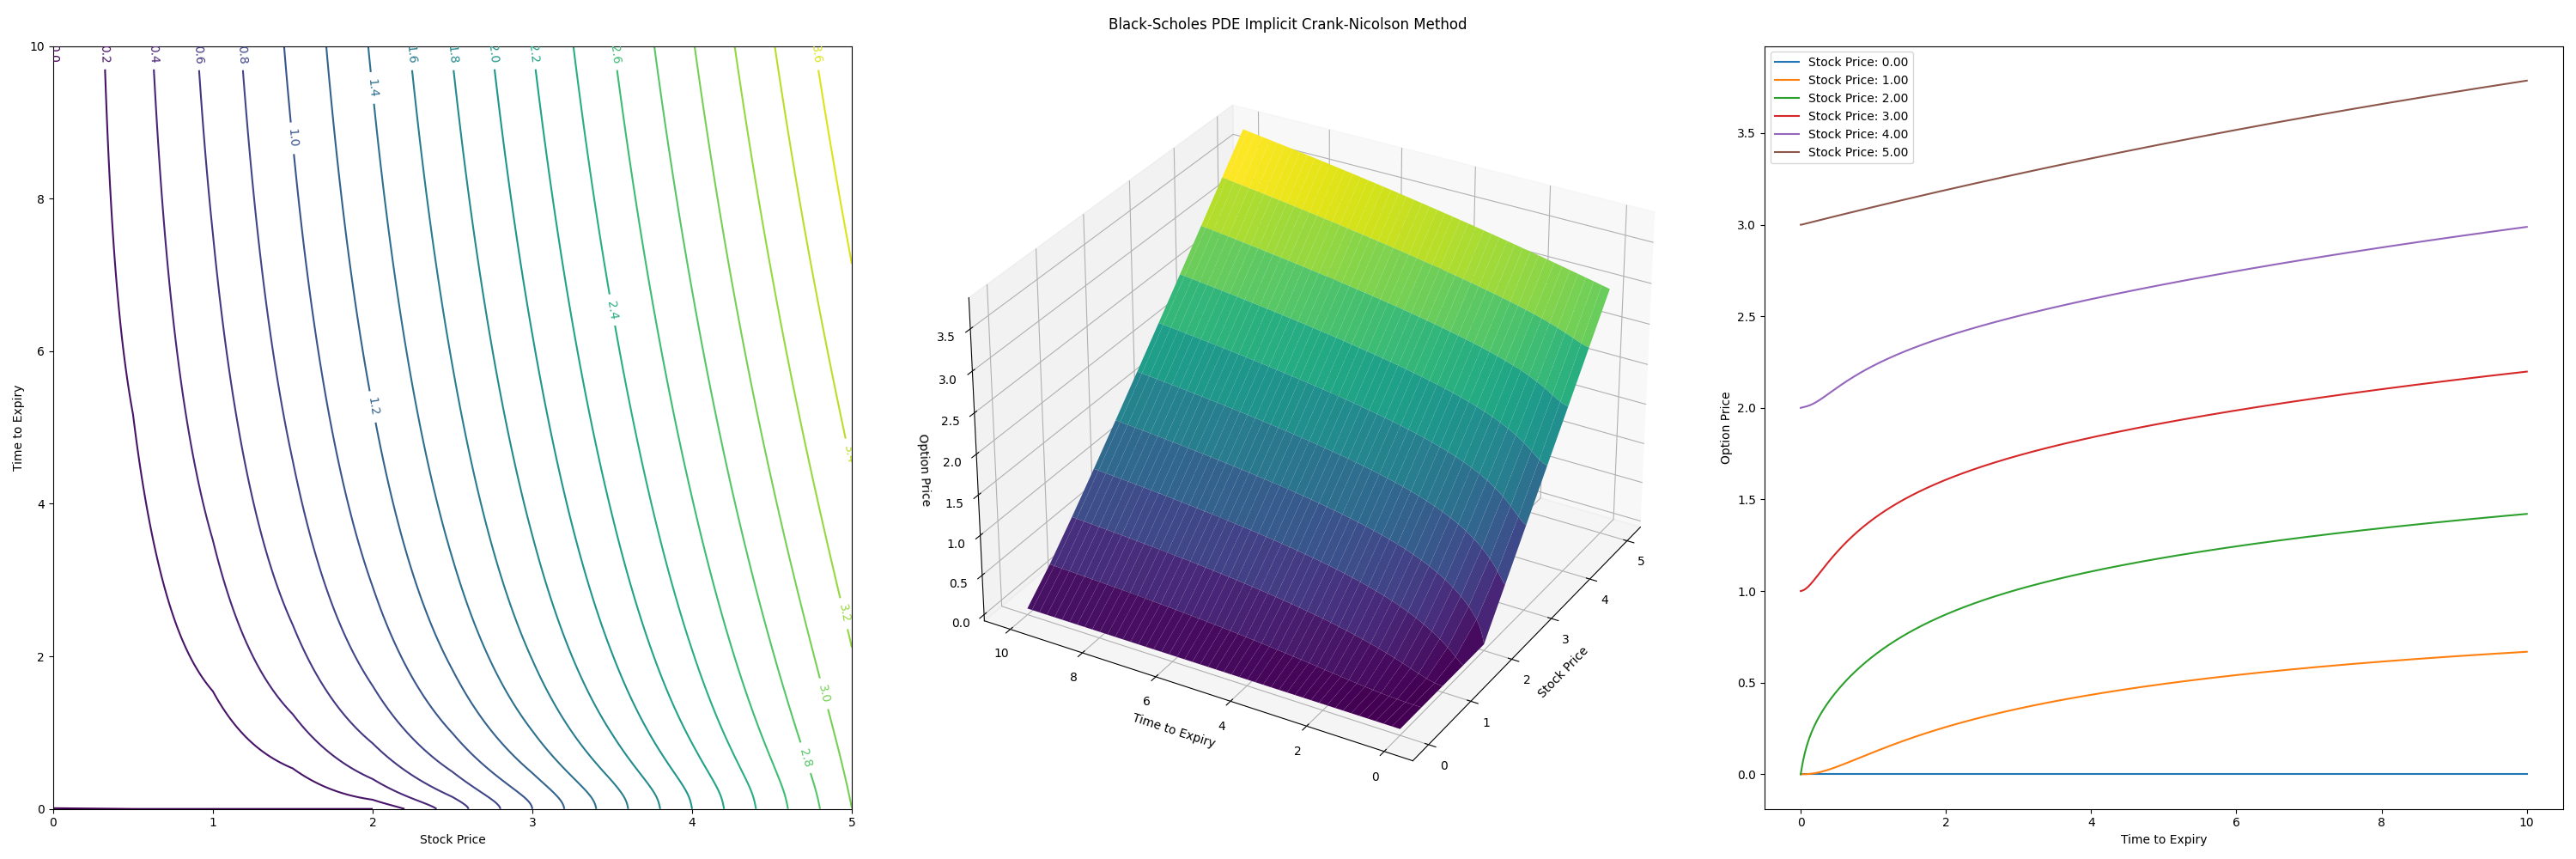
\includegraphics[width=0.8\textwidth]{implicit}
    \caption{Call option values using implicit method}
    \label{fig:implicit}
\end{figure}

\underline{Temporal Decrease}

All call option values $V$ decrease as the stock gets closer to maturity, regardless of stock price $S$. 
Lower stock prices experience a sharper drop closer to expiry while higher stock prices experience a gradual decrease when further from expiry and a less sudden drop closer to expiry. This is due to the discounted strike price effect (mathematically accounted for by the boundary condition: $V\left(S,\tau\right)\rightarrow S-Ke^{-r\tau}\ as\ S\ \rightarrow \infty$).

\underline{Value of Call Option upon expiry}\

Upon expiry, the call option $V$ is worth either the difference ($S-K$) between stock price $S$ and strike price $K$ (the amount originally paid for the option), or zero, whichever is higher. This is because a call option can only produce profit i.e. no losses are incurred regardless of the stock price.

\underline{Value of Call Option far from expiry}

When the expiry is sufficiently far away i.e. nowhere close to maturing, the call option value tends to its stock price $S$. 

\newpage
The grid was then made finer by using a smaller step in stock price of 0.01.

\begin{figure}[h]
    \centering
    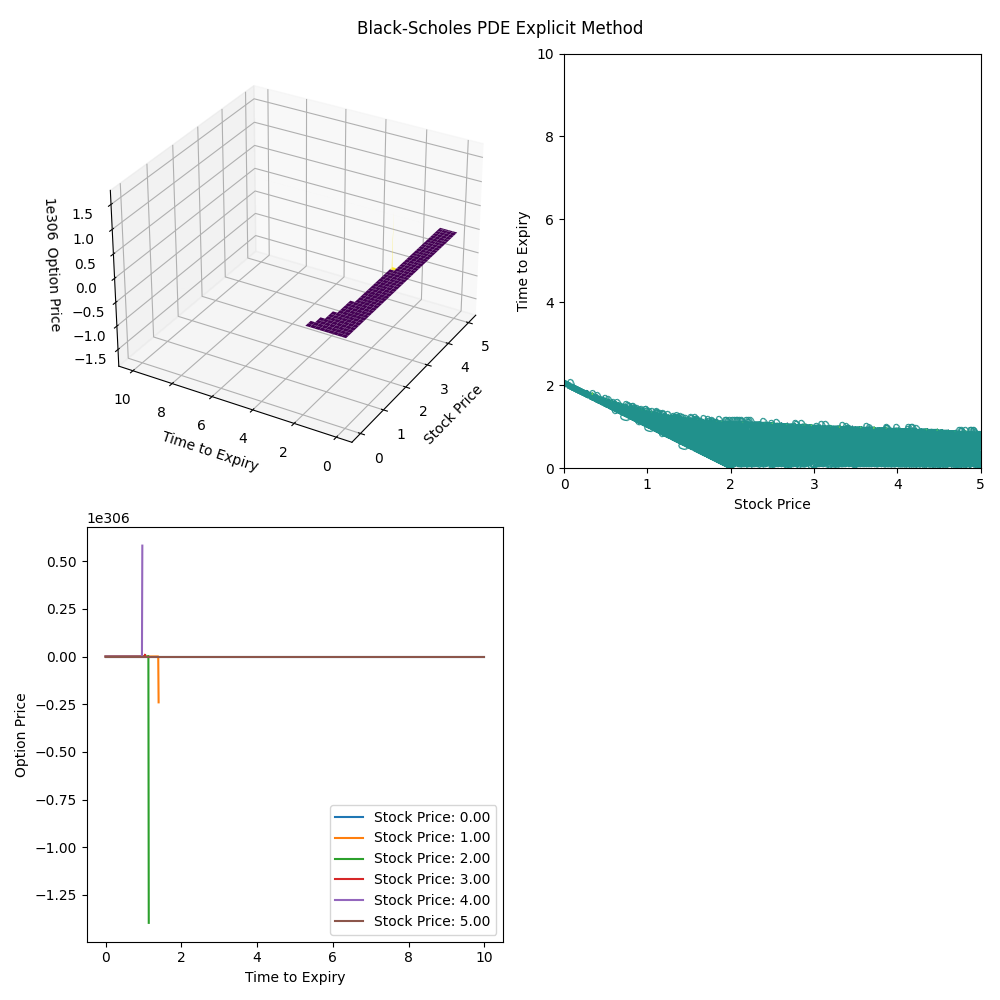
\includegraphics[width=0.8\textwidth]{explicit_fine}
    \caption{Call option values using explicit method with finer grid}
    \label{fig:explicit_fine}
\end{figure}

\underline{Explicit Method}

In the discretised equation, the weightage of the corresponding node at the prior time step $(V_{s,\tau})$ has to be positive i.e. 

\begin{equation}
    \frac{1}{k}-\frac{\sigma^2S^2}{h^2}-r>0
\end{equation}

This places a large constraint on the mesh size for stock price – with the parameters used in this coursework, mesh size $h \geq 0.5$ and time step $k \leq 0.01$  in order for the explicit method to be stable and use yield useful results. This constraint makes the explicit method largely impractical for precise determination of call option values. As evident in Figure \ref*{fig:explicit_fine}, the values are unstable and grow very large, failing to compute.

\newpage
\underline{Implicit Method}

\begin{figure}[h]
    \centering
    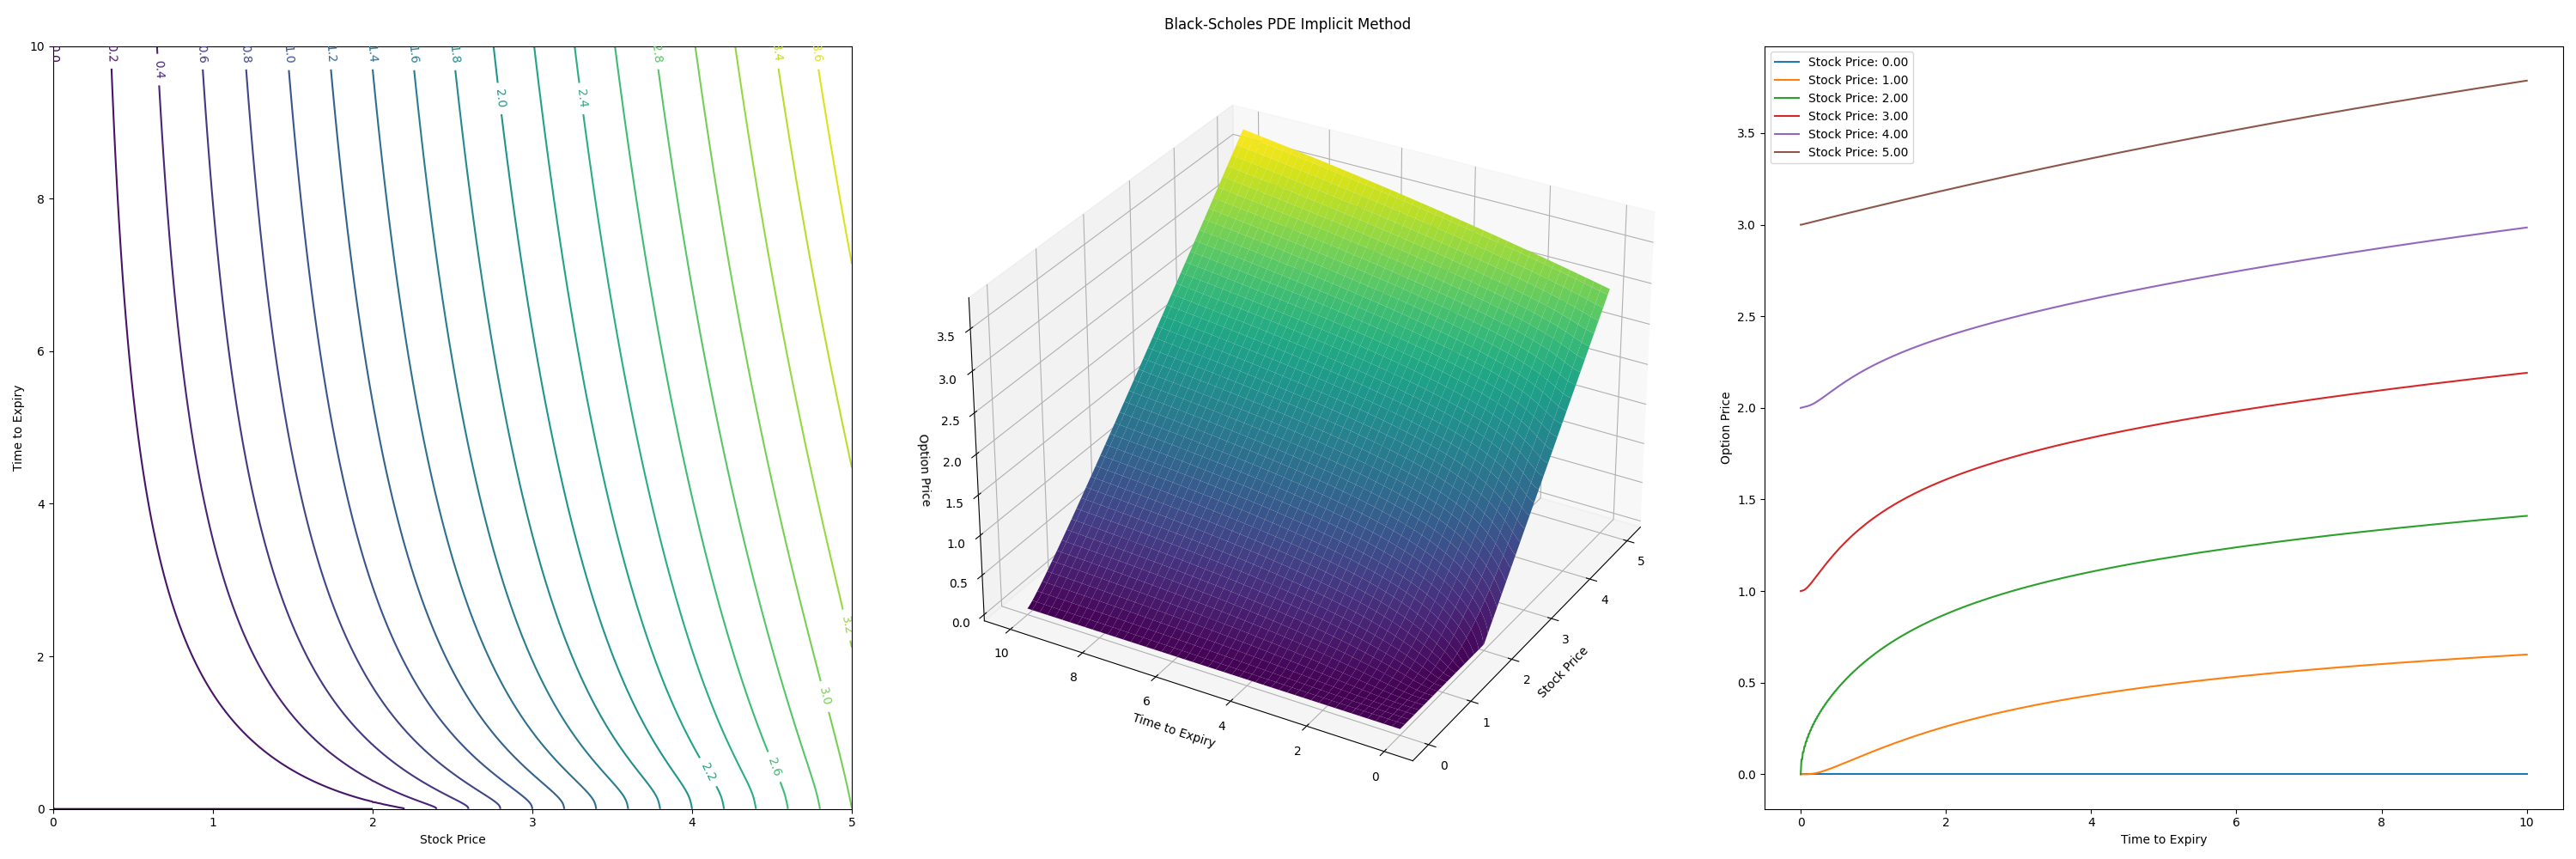
\includegraphics[width=0.8\textwidth]{implicit_fine}
    \caption{Call option values using implicit method with finer grid}
    \label{fig:implicit_fine}
\end{figure}

As Crank-Nicolson is an implicit method, mesh sizes and time steps are not constrained. A small mesh size $h$ and a reasonable time step $k$ can be used to determine call option values much more precisely. However, the implicit method requires much more computational power and time, to solve the system of equations using matrices. With a finer mesh resulting in a greater number of nodes, computational time increases exponentially and requires significantly more memory. 

\end{qn}

\begin{qn}{Other remarks (limits of the model, convergence problems, possible alternative approaches, anything you find relevant and important to mention):}
\underline{Alternative Methods}

As a possible alternative approach, the Black-Scholes PDE takes the form of a Cauchy-Euler equation and can therefore be converted to a diffusion equation by variable substitutions. Thereafter, the boundary conditions can be adapted to the diffusion equation and numerical solutions can be obtained. However, the additional change of variables step does not produce any particular advantage (other than the benefit of slightly less complex discretisation) and is hence not used in this case.

\end{qn}

\bibliography{cite}

\end{document}
